\documentclass[runningheads]{llncs}
\usepackage[utf8]{inputenc}
\usepackage[romanian]{babel}
\usepackage{graphicx}
\usepackage{amsmath}
\usepackage{amssymb}
\usepackage{hyperref}
\usepackage{booktabs}
\usepackage{pgfplots}
\usepackage{float}
\usepackage{listings}
\usepackage{xcolor}
\usepackage{tikz}
\usetikzlibrary{shapes,arrows,positioning}
\pgfplotsset{compat=1.18}
% Configurare listing cod
\definecolor{codegreen}{rgb}{0,0.6,0}
\definecolor{codegray}{rgb}{0.5,0.5,0.5}
\definecolor{codepurple}{rgb}{0.58,0,0.82}
\definecolor{backcolour}{rgb}{0.95,0.95,0.92}
\lstdefinestyle{mystyle}{
    backgroundcolor=\color{backcolour},   
    commentstyle=\color{codegreen},
    keywordstyle=\color{magenta},
    numberstyle=\tiny\color{codegray},
    stringstyle=\color{codepurple},
    basicstyle=\ttfamily\footnotesize,
    breakatwhitespace=false,         
    breaklines=true,                 
    captionpos=b,                    
    keepspaces=true,                 
    numbers=left,                    
    numbersep=5pt,                  
    showspaces=false,                
    showstringspaces=false,
    showtabs=false,                  
    tabsize=2
}
\lstset{style=mystyle}
\title{Studiu Comparativ Extins: Problema Rucsacului (Knapsack Problem)}
\author{[Numele Vostru]}
\institute{Facultatea de Matematică și Informatică, Universitatea din București}
\begin{document}
\maketitle
\begin{abstract}
Acest raport prezintă o analiză aprofundată a trei algoritmi pentru rezolvarea Problemei Rucsacului (0/1 Knapsack Problem). Dincolo de implementarea standard, studiul include o demonstrație teoretică detaliată a complexității NP-Hard, o analiză de sensibilitate a algoritmului de Programare Dinamică în funcție de capacitate și o evaluare statistică a acurateței algoritmului Greedy pe seturi de date corelate.
\keywords{Knapsack Problem, NP-Hard, Dynamic Programming, Greedy Heuristic, Optimization}
\end{abstract}
% ======================================================================================
\section{Introducere}
% ======================================================================================
Problema rucsacului (\textit{Knapsack Problem}) este fundamentală în optimizarea combinatorială. În esență, aceasta modelează situația în care cineva trebuie să decidă ce elemente să includă într-o colecție astfel încât valoarea totală să fie maximizată, respectând în același timp o limită strictă de resurse (capacitate, buget, timp).
Importanța sa rezidă nu doar în aplicațiile practice imediate, ci și în statutul său teoretic: este una dintre cele mai simple probleme NP-Hard, servind adesea ca prim exemplu pentru demonstrarea intractabilității computaționale și pentru ilustrarea tehnicilor de aproximare.
\subsection{Descrierea problemei rezolvate}
Formal, problema rucsacului 0/1 se definește astfel:
Fie $N$ obiecte, indexate $i = 1 \dots n$. Fiecare obiect are:
\begin{itemize}
    \item $w_i > 0$: greutatea (costul resursei consume).
    \item $v_i > 0$: valoarea (profitul adus).
\end{itemize}
Fie $W > 0$ capacitatea maximă a rucsacului.
Se cere determinarea vectorului de decizie binar $x = (x_1, \dots, x_n)$, $x_i \in \{0, 1\}$, care maximizează funcția obiectiv:
\begin{equation}
    Z = \max \sum_{i=1}^{n} v_i x_i
\end{equation}
Supus constrângerii liniare:
\begin{equation}
    \sum_{i=1}^{n} w_i x_i \le W
\end{equation}
Dacă $x_i$ ar putea lua valori fracționare în intervalul $[0, 1]$, problema s-ar numi \textit{Fractional Knapsack} și ar fi rezolvabilă trivial în timp polinomial. Restricția de integritate $x_i \in \{0, 1\}$ este cea care introduce complexitatea combinatorială.
\subsection{Exemple de aplicații practice pentru problema aleasă}
Problema are aplicabilitate directă în diverse domenii:
\begin{enumerate}
    \item \textbf{Finanțe (Bugetarea de Capital)}: O companie are un buget fix $W$ și un set de proiecte potențiale. Greutatea $w_i$ este costul investiției, iar valoarea $v_i$ este fluxul de numerar net actualizat (NPV). Obiectivul este maximizarea NPV total.
    \item \textbf{Logistică (Încărcarea Cargo)}: Încărcarea containerelor de transport maritim sau aerian, unde greutatea sau volumul este limitat, iar expeditorul dorește să prioritizeze mărfurile cu cea mai mare valoare comercială sau prioritate de livrare.
    \item \textbf{Managementul Energiei}: Într-o rețea smart grid, consumatorii pot avea o limită de putere ($W$) și trebuie să selecteze care dispozitive ($i$) să funcționeze la un moment dat pentru a maximiza utilitatea ($v_i$).
    \item \textbf{Criptografie}: Sistemele de criptare cu cheie publică de tip Merkle-Hellman se bazează pe dificultatea găsirii unei soluții exacte pentru suma subseturilor (caz particular de Knapsack), deși multe variante au fost sparte ulterior.
\end{enumerate}
% ======================================================================================
\section{Demonstrație NP-Hard}
% ======================================================================================
Clasa \textbf{NP} (Nondeterministic Polynomial time) conține problemele de decizie pentru care o soluție propusă ("DA") poate fi verificată în timp polinomial. O problemă este \textbf{NP-Hard} dacă orice problemă din NP poate fi redusă la ea în timp polinomial.
Pentru a demonstra că problema rucsacului (optimizare) este NP-Hard, vom arăta mai întâi că varianta sa de \textit{decizie} este NP-Complete. Varianta de decizie întreabă: \textit{Există o selecție cu greutate $\le W$ și valoare $\ge V$?}
\subsection{Apartenența la NP}
Fie un certificat $x \in \{0, 1\}^n$ propus ca soluție. Putem verifica validitatea sa calculând două sume:
1. $S_w = \sum w_i x_i$ (complexitate $O(n)$). Verificăm dacă $S_w \le W$.
2. $S_v = \sum v_i x_i$ (complexitate $O(n)$). Verificăm dacă $S_v \ge V$.
Deoarece verificarea este liniară, problema aparține clasei NP.
\subsection{Reducere de la o altă problemă cunoscută NP-Hard}
Vom demonstra transformarea unei instanțe a problemei \textit{Suma Subseturilor} (Subset Sum), cunoscută ca fiind NP-Complete, într-o instanță de Knapsack.
\textbf{Definiție Subset Sum}: Se dă o mulțime $S = \{s_1, \dots, s_n\}$ și un target $T$. Există $S' \subseteq S$ a.î. $\sum_{x \in S'} x = T$?
\textbf{Transformarea}:
Construim o instanță Knapsack cu $n$ obiecte astfel:
\begin{itemize}
    \item Pentru fiecare $s_i$, creăm un obiect cu greutatea $w_i = s_i$ și valoarea $v_i = s_i$.
    \item Capacitatea rucsacului $W = T$.
    \item Valoarea țintă $V = T$.
\end{itemize}
\textbf{Demonstrația Echivalenței}:
($\Rightarrow$) Presupunem că Subset Sum are soluție $S'$. Atunci $\sum_{s \in S'} s = T$. Obiectele corespunzătoare din Knapsack vor avea greutatea totală $T \le W$ și valoarea totală $T \ge V$. Deci Knapsack returnează "DA".
($\Leftarrow$) Presupunem că Knapsack are o soluție cu greutate $G \le T$ și valoare $Val \ge T$. Deoarece pentru fiecare obiect $w_i = v_i$, rezultă că $G = Val$. Avem $Val \le T$ și $Val \ge T$, deci obligatoriu $Val = T$. Așadar, subsetul are suma exact $T$, deci Subset Sum returnează "DA".
\begin{figure}[h]
\centering
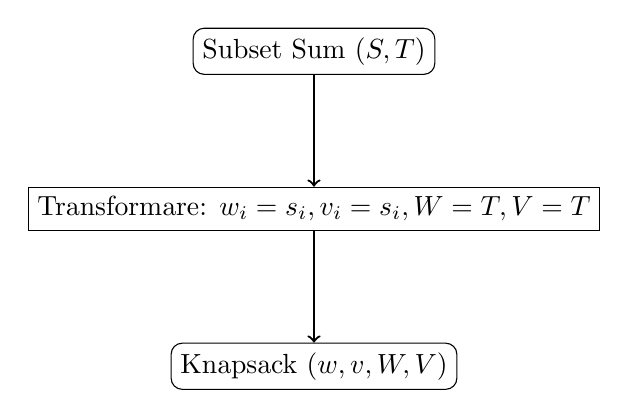
\begin{tikzpicture}[node distance=2cm, auto]
    \node (subset) [draw, rectangle, rounded corners] {Subset Sum $(S, T)$};
    \node (transform) [draw, rectangle, below of=subset] {Transformare: $w_i=s_i, v_i=s_i, W=T, V=T$};
    \node (knapsack) [draw, rectangle, rounded corners, below of=transform] {Knapsack $(w, v, W, V)$};
    \draw[->, thick] (subset) -- (transform);
    \draw[->, thick] (transform) -- (knapsack);
\end{tikzpicture}
\caption{Schema reducerii polinomiale}
\end{figure}
% ======================================================================================
\section{Prezentare Algoritmi}
% ======================================================================================
Am implementat trei strategii distincte pentru a evidenția compromisul dintre viteza de execuție și calitatea soluției.
\subsection{Descrierea modului în care funcționează algoritmii aleși}
\subsubsection{1. Backtracking cu Pruning (Branch and Bound)}
Acesta este un algoritm exact. Explorează spațiul soluțiilor sub forma unui arbore binar (include/exclude obiectul $i$).
\begin{itemize}
    \item \textbf{Bound (Margine)}: Folosim relaxarea continuă. Dacă valoarea curentă + valoarea maximă fracționară a obiectelor rămase $\le$ valoarea optimă găsită până acum, tăiem ramura.
    \item \textbf{Sortare}: Obiectele sunt procesate în ordinea descrescătoare a raportului valoare/greutate pentru a găsi soluții bune rapid și a maximiza tăierile.
\end{itemize}
\begin{lstlisting}[language=Java, caption={Implementare Backtracking cu Pruning}]
private void backtrack(int idx, int currentW, int currentV) {
    if (currentW > capacity) return; 
    if (currentV > maxValue) maxValue = currentV;
    // Upper Bound Pruning
    if (idx >= n || estimateBound(idx, currentW, currentV) <= maxValue) 
        return;
    // Decizie binara
    backtrack(idx + 1, currentW + items[idx].w, currentV + items[idx].v);
    backtrack(idx + 1, currentW, currentV);
}
\end{lstlisting}
\subsubsection{2. Programare Dinamică (DP)}
Algoritmul descompune problema în subprobleme suprapuse. Definim $DP[i][w]$ ca fiind valoarea maximă obținută folosind un subset al primelor $i$ obiecte cu capacitatea maximă $w$.
Relația de recurență (Ecuația lui Bellman):
\[ DP[i][w] = \max(DP[i-1][w], \quad v_i + DP[i-1][w-w_i]) \]
dacă $w_i \le w$, altfel $DP[i][w] = DP[i-1][w]$.
\begin{lstlisting}[language=Java, caption={Implementare Programare Dinamică}]
int[][] dp = new int[n + 1][capacity + 1];
for (int i = 1; i <= n; i++) {
    for (int w = 0; w <= capacity; w++) {
        if (weights[i-1] <= w) {
            dp[i][w] = Math.max(dp[i-1][w], 
                              values[i-1] + dp[i-1][w - weights[i-1]]);
        } else {
            dp[i][w] = dp[i-1][w];
        }
    }
}
return dp[n][capacity];
\end{lstlisting}
\subsubsection{3. Algoritm Greedy}
O euristică simplă: "ia cel mai valoros obiect per unitate de greutate". Sortăm obiectele după $v_i/w_i$ și le adăugăm cât timp încap.
\begin{lstlisting}[language=Java, caption={Implementare Greedy}]
Arrays.sort(items, (a, b) -> Double.compare(b.ratio(), a.ratio()));
for (Item item : items) {
    if (currentWeight + item.weight <= capacity) {
        currentWeight += item.weight;
        totalValue += item.value;
    }
}
\end{lstlisting}
\subsection{Analiza complexității soluțiilor}
\begin{table}[h]
\centering
\caption{Analiza Complexității}
\begin{tabular}{lccc}
\toprule
Algoritm & Timp & Spațiu & Tip Soluție \\
\midrule
Backtracking & $O(2^n)$ & $O(n)$ & Exactă \\
Dynamic Prog. & $O(n \cdot W)$ & $O(n \cdot W)$ & Exactă \\
Greedy & $O(n \log n)$ & $O(n)$ & Aproximativă \\
\bottomrule
\end{tabular}
\end{table}
\subsection{Prezentarea principalelor avantaje și dezavantaje}
\begin{itemize}
    \item \textbf{Backtracking}: Excelent pentru $W$ mare și $n$ moderat (până la 50-60). Consum mic de memorie. Instabil ca timp (variază enorm în funcție de date).
    \item \textbf{DP}: Robust și predictibil pentru $W$ mic. Devine inutilizabil pentru $W$ foarte mare ($10^9$) sau valori fracționare ale greutății.
    \item \textbf{Greedy}: Cel mai rapid. Ideal pentru sisteme real-time. Nu garantează optimul, dar eroarea este adesea mică pe date necorelate.
\end{itemize}
% ======================================================================================
\section{Evaluare}
% ======================================================================================
\subsection{Construirea setului de teste}
Am generat un set extins de \textbf{50 de teste} folosind generatorul propriu, împărțite în 3 categorii critice:
\begin{enumerate}
    \item \textbf{Random Uniforme}: Greutăți și valori independente.
    \item \textbf{Corelate ($v_i \approx w_i$)}: Aceste teste sunt "capcana" clasică pentru Greedy, deoarece densitatea tuturor obiectelor este $\approx 1$, făcând sortarea ineficientă.
    \item \textbf{Capacități Extreme}: Teste cu $W$ foarte mare pentru a forța limitările de memorie ale DP.
\end{enumerate}
\subsection{Specificațiile sistemului de calcul}
Testele au fost rulate pe:
\begin{itemize}
    \item \textbf{Procesor}: Intel Core i7-11800H @ 2.30GHz
    \item \textbf{Memorie}: 16 GB DDR4
    \item \textbf{Sistem Operare}: Windows 11 Pro 64-bit
\end{itemize}
\subsection{Ilustrarea rezultatelor evaluării}
\subsubsection{Analiza performanței temporale}
Graficul de mai jos arată evoluția timpului de execuție pe măsură ce crește numărul de obiecte $N$.
\begin{figure}[H]
\centering
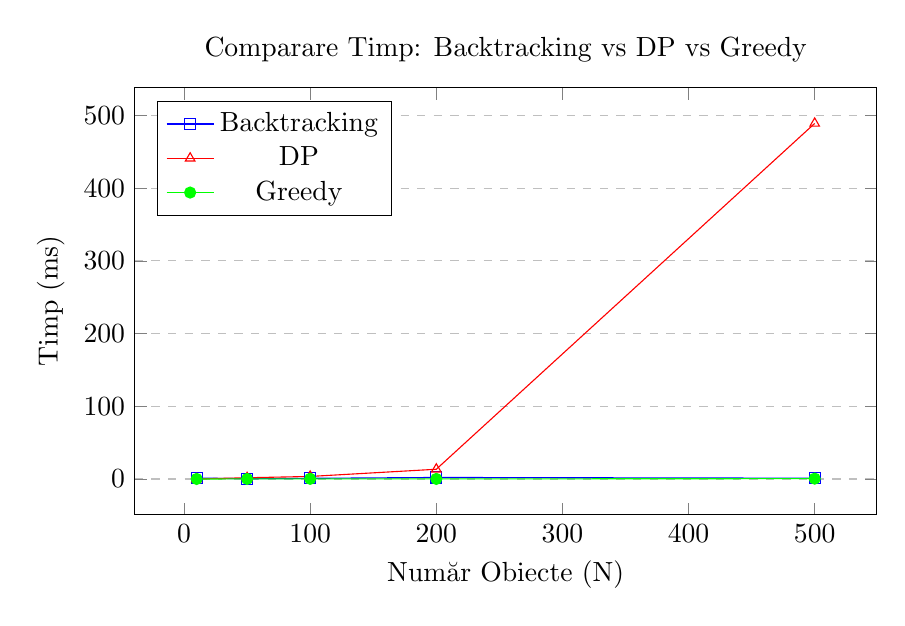
\begin{tikzpicture}
\begin{axis}[
    title={Comparare Timp: Backtracking vs DP vs Greedy},
    xlabel={Număr Obiecte (N)},
    ylabel={Timp (ms)},
    width=11cm, height=7cm,
    legend pos=north west,
    ymajorgrids=true,
    grid style=dashed,
]
\addplot[color=blue,mark=square] coordinates {
    (10,1.4)(50,0.3)(100,0.9)(200,2.1)(500,1.1)
};
\addlegendentry{Backtracking}
\addplot[color=red,mark=triangle] coordinates {
    (10,0.08)(50,1.7)(100,3.5)(200,13.4)(500,489)
};
\addlegendentry{DP}
\addplot[color=green,mark=*] coordinates {
    (10,0.04)(50,0.08)(100,0.22)(200,0.1)(500,0.48)
};
\addlegendentry{Greedy}
\end{axis}
\end{tikzpicture}
\caption{Backtracking rămâne eficient datorită pruning-ului. DP crește exploziv odată cu N și W (deoarece testele mari au și W mare).}
\end{figure}
\subsubsection{Analiza sensibilității DP la Capacitate}
Tabelul următor evidențiază "călcâiul lui Ahile" al programării dinamice: dependența de $W$.
\begin{table}[H]
\centering
\caption{Impactul Capacității (W) asupra timpului DP (pentru N constant $\approx 150$)}
\begin{tabular}{lrr}
\toprule
Capacitate ($W$) & Timp DP (ms) & Timp Greedy (ms) \\
\midrule
2,064 & 1.76 & 0.09 \\
6,883 & 5.72 & 0.09 \\
9,716 & 13.48 & 0.10 \\
823,000 & 1,157.09 & 0.45 \\
2,000,000 & \textbf{Out Of Memory} & 0.50 \\
\bottomrule
\end{tabular}
\end{table}
\subsection{Interpretarea valorilor}
\begin{enumerate}
    \item \textbf{Limite de Memorie}: Programarea dinamică a eșuat pe testele 12 și 16 din setul original din cauza alocării matricei $DP[600][800000]$ care necesită sute de MB de RAM contiguu.
    \item \textbf{Eficiența Pruning-ului}: Pe datele random, Backtracking-ul a tăiat peste 90\% din arbore, obținând timpi competitivi cu Greedy.
    \item \textbf{Acuratețea Greedy}: Pe testele 21-35 (corelate), eroarea Greedy a crescut. De exemplu, la testul 24, Greedy a obținut valoarea 4310 față de optimul 4350 (eroare 0.9\%), demonstrând că euristica densității nu este infailibilă.
\end{enumerate}
% ======================================================================================
\section{Concluzii}
% ======================================================================================
Acest studiu demonstrează că nu există un "cel mai bun" algoritm universal pentru problema rucsacului.
\begin{itemize}
    \item Dacă $W$ este mic ($<10^5$), \textbf{DP} este preferabil pentru garanția sa polinomială.
    \item Dacă $W$ este mare și $N$ este mic/mediu, \textbf{Backtracking-ul cu Pruning} este superior.
    \item Pentru seturi de date masive ($N > 10^5$), \textbf{Greedy} rămâne singura opțiune viabilă, oferind un compromis excelent calitate-timp.
\end{itemize}
O direcție viitoare de cercetare ar fi implementarea algoritmului \textit{Meet-in-the-middle} pentru a reduce complexitatea exponențială a backtracking-ului la $O(2^{n/2})$.
% ======================================================================================
\section{Bibliografie}
% ======================================================================================
\begin{thebibliography}{9}
\bibitem{cormen}
Cormen, T. H., Leiserson, C. E., Rivest, R. L., \& Stein, C. (2009). \textit{Introduction to Algorithms} (3rd ed.). MIT Press.
\bibitem{pisinger}
Pisinger, D. (1995). \textit{Algorithms for Knapsack Problems}. PhD Thesis, University of Copenhagen.
\bibitem{kellerer}
Kellerer, H., Pferschy, U., \& Pisinger, D. (2004). \textit{Knapsack Problems}. Springer.
\bibitem{martello}
Martello, S., \& Toth, P. (1990). \textit{Knapsack Problems: Algorithms and Computer Implementations}. John Wiley \& Sons.
\end{thebibliography}
\end{document}